\chapter{Edge classification}
\label{chap:gnn}

Graphs constructed by both methods introduced in the last chapter contain many fake edges.
The second stage of the GNN4ITk chain labels the graph connections, so that fake ones are removed and track candidates are built from exclusively true connections. 
We carry out this task using a Graph Neural Network (GNN), which leverages the graph connectivity to compute a score for each edge that represents the probability of being a true edge.
This chapter describes the edge classification stage, starting with a general introduction to GNNs.
Sections \ref{sect:chap-gnn-filter-network} and \ref{sect:ignn} respectively detail the filter network and the interaction network, two edge-classifying GNN architectures investigated in this thesis, and their results. 

\section{Introduction to graph neural networks}
\label{sect:chap-gnn-intro-to-graph-network}

The last 15 years have seen an explosion of deep neural networks into a major domain of machine learning, achieving unprecedented performance on complicated tasks thanks to increasingly available training data and computing power. 
An ecosystem of different network architectures has been explored targeting different data representations. 
For example, Feed-forward Neural Networks (FNNs) for tabular data, Convolutional Neural Networks (CNNs) for 2-dimensional images, Recurrent Neural Networks (RNNs) for sequences.
These architectures are effective on Euclidean, or grid-like data, but not sufficiently flexible to model irregular non-Euclidean data structures such as graphs, which comprise entities (nodes) and their relationships (edges). 
In this context, \textbf{Graph Neural Networks} enable representation learning on graph-structured data by leveraging the underlying patterns in features associated with nodes and edges.

Graph neural networks operate on a graph by iteratively propagating information via the edges.
The representation of a node is updated based on its features and those of its direct neighbours through a learnable aggregation mechanism.
The general formulation of the $k$-th iteration at can be written as 
\beq
\label{eq:gnn:1}
\mathbf{h}_i^k = \mathrm{UPDATE}_k \left( \mathbf{h}_i^{k-1}, \mathrm{AGGREGATE}_k\left( \{\mathbf{h}_j ^{k-1} : j\in \mathcal{N} (v_i) \} \right) \right)
\eeq
where $\mathbf{h}_i^k$ denotes the embedding of node $v_i$ after the $k$-th iteration, and $\mathcal{N} (v_i)$ the set of neighbouring nodes of $v_i$. 
Numerous GNN architectures have been proposed, from the simple Graph Convolutional Networks (GCNs) \cite{gcn}, which leverage spectral graph theory to define convolution-like operations on graphs, Graph Attention Networks (GATs) \cite{gat}, which introduce attention mechanisms for adaptive neighbourhood weighting, to GraphSAGE \cite{graphsage}, and Graph Isomorphism Networks (GINs) \cite{gin}, which improved expressiveness in distinguishing graph structures.

\section{The filter network}
\label{sect:chap-gnn-filter-network}

In the previous section, we have motivated and introduced graph neural networks as the deep learning method for non-Euclidean data represented as graphs. 
The GNN4ITk algorithm uses graph networks to identify fake edges in the graphs built from the methods described in chapter \ref{chap:graph-construction}. 

\subsection{Method}

As discussed in \ref{subsect:metric-learning} and shown on figure \ref{fig:metric-learning-efficiency}, the number of edges in a graph produced by the \textbf{Metric Learning} method is on average $\abs{E} = (6.92\pm0.17)\times 10^6$, most of which are fake. 
For comparison, the number of true target edges are of $\mathcal{O}(10^4)$, two orders of magnitude fewer. 
% In addition, not all fake edges are created equal.
Among the fake edges, we can categorize \textit{hard} fake edges as those resembling true edges, for example, a connection from a source node $i$ to a false destination node $j'$ on the same detector module as the true destination node $j$, so that $\abs{\mathbf{r}_j - \mathbf{r}_{j'}} \approx 0$. 
The true edge $e_{ij}$ is therefore difficult to distinguish from the fake edge $e_{ij'}$.
In contrast, \textit{easy} fakes are recognizable from target true edges, such as unphysical edges randomly selected by the kNN. 

% The high number of fake edges creates a severe imbalance in the two classes, and more importantly, directs the edge classifier's focus away from hard fakes. 
Because hard fakes are difficult to identify, it is necessary to train a deep network to guarantee good performance. 
A large graph coupled with a large network creates a bottleneck in inference time and resource consumption. 
In addition, training on both hard and easy fake edges directs the classifier's attention away from hard fakes and affects the performance.
% As inference time and resources approximately scale with graph size, the large number of edges presents a bottleneck in production. 
A better strategy, therefore, is to train a shallow network on the output graphs of the Metric Learning to eliminate easy fakes and subsequently a deeper, more sophisticated network to eliminate hard fakes. 
The first network, designated the \textbf{Filter Network}, is described in this section, and the second, called the \textbf{Interaction Network}, in section \ref{sect:ignn}.

The architecture of the Filter Network is based on the \graphsage~convolution proposed by reference \cite{graphsage}, which facilitates the efficient learning of large complex graphs.
The idea is to train a set of functions which aggregate and propagate information between different depths of a node's neighborhood.
We define a $k$-hop neighborhood of a node as the subset of nodes whose shortest path to the center node proceeds through exactly $k$ edges.
Figure \ref{fig:filter-sage} shows an example of a \textcolor{reddish}{central node} and its neighborhoods with $k=1$ and $k=2$.
% For example, around the \textcolor{reddish}{ central } node in figure \ref{fig:filter-sage}, we define a k-hope neighborhood as the subset of nodes whose shortest path to the \textcolor{reddish}{}.
% For each search depth $k$, a function aggregates information from the corresponding nodes. 
At each depth, a trainable function aggregates the features of the nodes residing within, and passes the aggregated features to the next depth.
In the figure, the messages from \textcolor{darkgreen}{nodes} at $k=2$ gathered by the \textcolor{darkgreen}{\textbf{ green aggregator}} are used to evolve the features of \textcolor{darkblue}{\textbf{nodes}} at $k=1$, which are then aggregated by the \textcolor{darkblue}{blue aggregator} and passed to the \textcolor{reddish}{central node}.

\begin{figure}[h!]
    \centering
    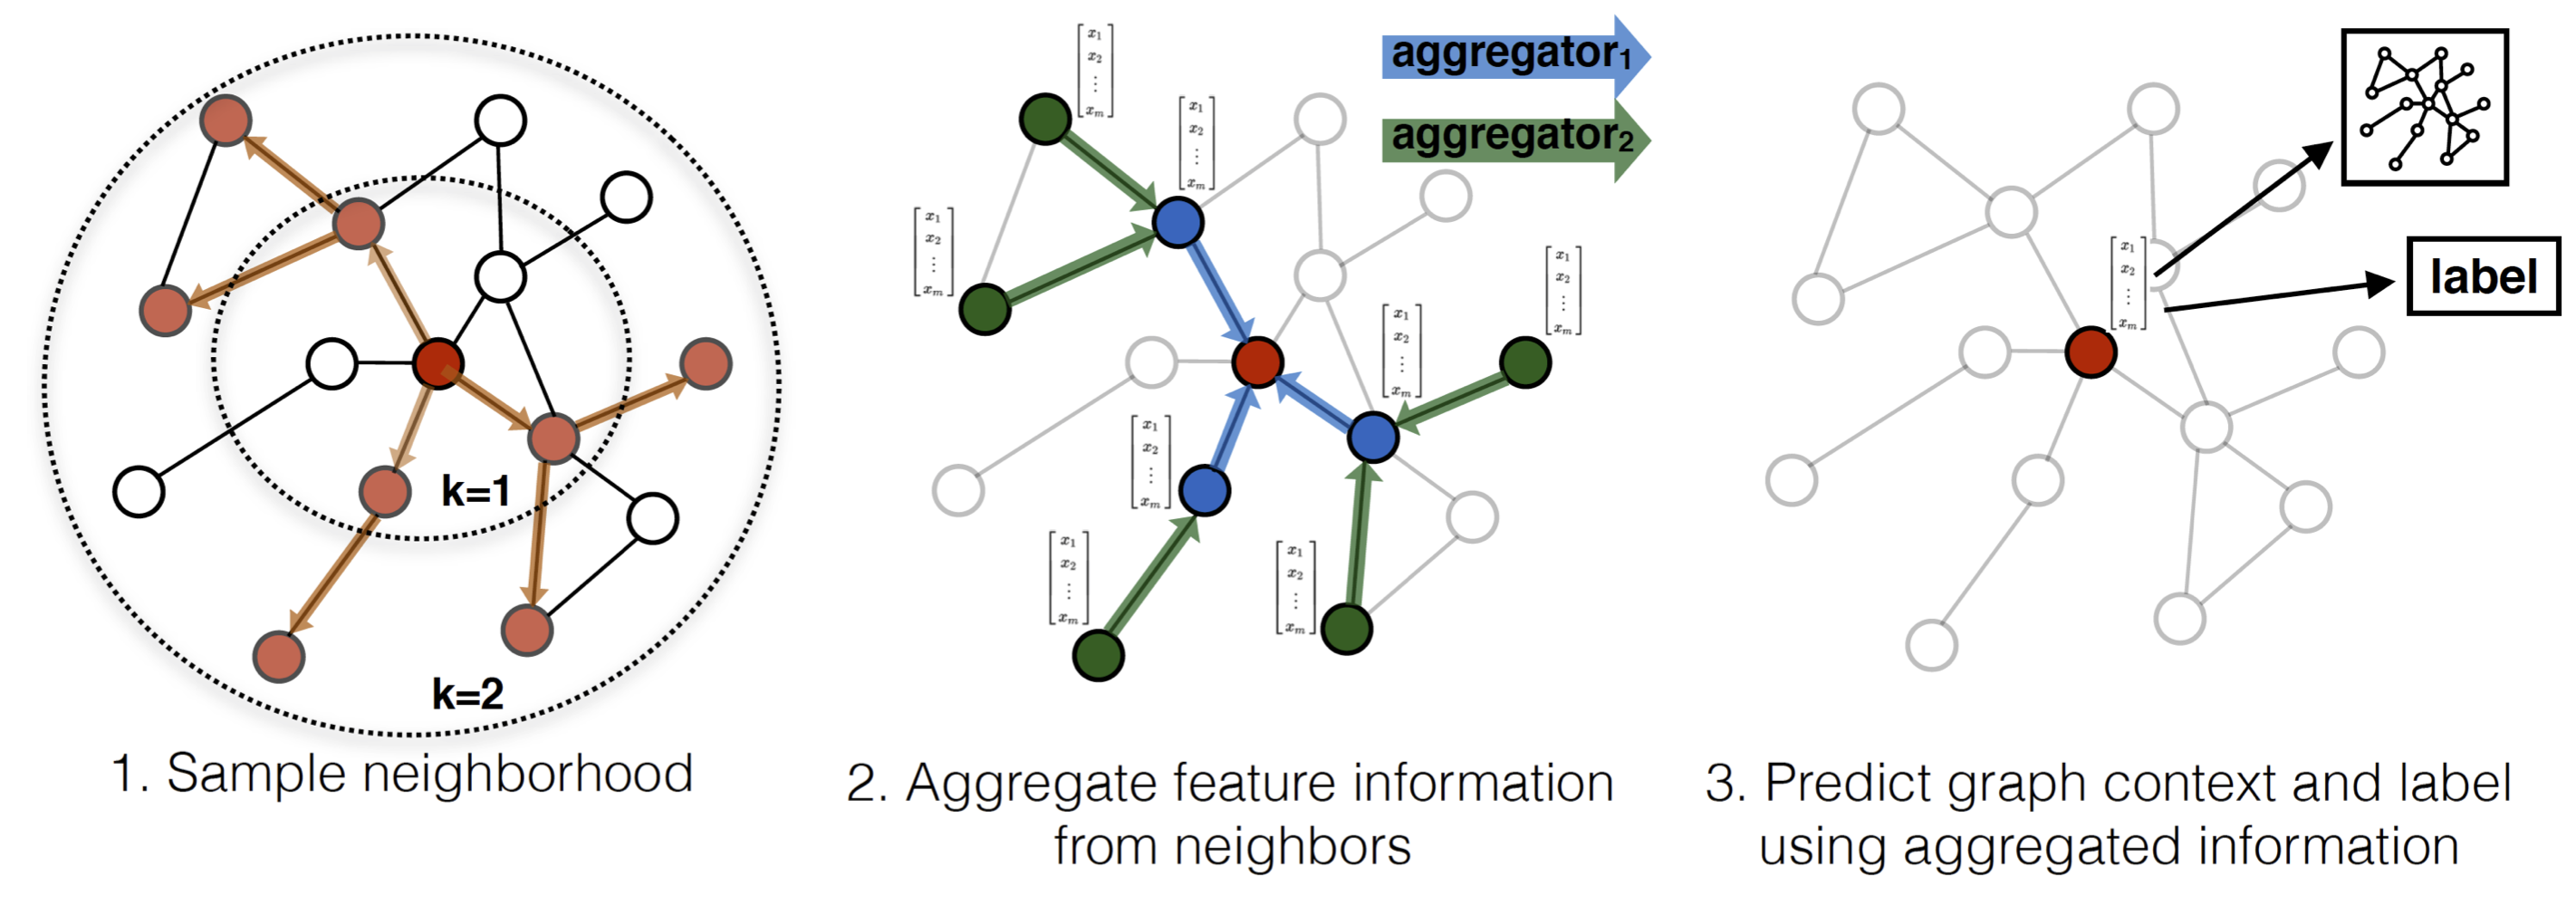
\includegraphics[width=0.8\textwidth]{figures/sample_and_agg.png}
    \caption{\graphsage~ sampling and aggregation mechanism. \cite{graphsage}}
    \label{fig:filter-sage}
\end{figure}

This mechanism is expressed more concretely in the pseudocode shown in algorithm \ref{alg:sage}. 
Each \graphsage~is defined by $K$ aggregator functions, denoted $\text{AGGREGATE}_k,\,k\in\{1,\dotsc,K\}$, and a set of weight matrices $\mathbf{W}^k,\,k\in\{1,\dotsc,K\}$, which propagate the aggregated information between different search depths.
The aggregators must be differentiable to allow back-propagation through the search depths.
% transforms node input vector into node embedding taking into account the information aggregated from the local neighbourhood, assuming a fully trained model.
Recall that the graph is defined by a set of nodes $V$ and a set of edges $E$. 
To each node $i\in V$ is associated a node feature vector $\mathbf{x}_i\in\mathbb{R}^{d}$. 
A neighbourhood function $\mathcal{N}: v\rightarrow {V}$ finds other nodes directly connected to a given node $v$.
\begin{algorithm}
\caption{Calculation of node embedding $\mathbf{z}_i$ with \graphsage~\cite{graphsage} }\label{alg:sage}
$h^0_{i} \gets \mathbf{x}_i$\;
\For{$k \in \{1,\dotsc K\}$}{
  \For{$i\in \{1,\dotsc, \abs{V}\}$}{
    $\mathbf{h}^k_{\mathcal{N}(v_i)} \gets \textsc{Aggregate} _k (\{ \mathbf{h}_j^{k-1} \, \forall  v_j \in \mathcal{N}(v_i) \} )$ ; \\
    $\mathbf{h}_i^k  \gets \sigma \left(\mathbf{W}^k\cdot [\mathbf{h}_v^{k-1}|\mathbf{h}^k_{\mathcal{N}(v_i)}] \right)$
  }
  $\mathbf{h}_i^k  \gets \frac{\mathbf{h}_i^k}{\norm{\mathbf{h}_i^k} _2}, \, \forall v_i \in \mathcal{V}$
}
$\mathbf{z}_i \gets \mathbf{h}_i^K \, \forall v_j \in \mathcal{V},$\\
where $\sigma(\cdot)$ is an activation function, $[\mathbf{x} | \mathbf{y}]$ a vector concatenation.
\end{algorithm}
In each step $k$, to each node $v_i \in \mathcal{V}$ are aggregated the representations of other nodes in its local neighborhood $\{ \mathbf{h}_j^{k-1} \}$, found by $\mathcal{N}(v_i)$, into a single vector $\mathbf{h}^k_{\mathcal{N}(v_i)}$. 
The current representation of $v_i$ namely $\mathbf{h}_v^{k-1}$ is concatenated with $\mathbf{h}^k_{\mathcal{N}(v_i)}$, and fed through an MLP represented by $W^k$, followed by a non-linear activation function $\sigma$.
As this process iterates, nodes incrementally receive more information from further reaches of the graph, and their features become more expressive.
% The resulted representation $\mathbf{h}_i^k$ is normalized and becomes the input to the next step. 
% The output node embedding is the normalized representation at depth $K$.

Any element-wise function is a good aggregator. 
However, for simplicity the \textbf{Filter} uses the mean aggregator, i.e.
\begin{equation}
    \label{eq:10.1}
    \textsc{Aggregate}\left( \{ \mathbf{h}_1 ,\dotsc  \mathbf{h}_N \}\right) = \frac{1}{N} \sum_{i=1} ^N \mathbf{h}_i
\end{equation}

The neighbourhood function $\mathcal{N}(v)$ uniformly draws a fixed number of edges from the set $\{(u,v)\in \mathcal{V} \}$, instead of using the entire $1$-hop neighbourhood.
Sampling limits the memory footprint of a \graphsage~operation on large graphs. 
Without it, the consumption becomes unpredictable and grows with $\abs{\mathcal{V}}$.
It is found in reference \cite{graphsage} that $K=2$ and sample sizes $S_1=25$, $S_2=10$ produce a good balance between memory and performance, which are used in the \textbf{Filter}.

With the \graphsage~mechanism defined, we can now describe the network architecture. 
First, the node embedding is evolved over $L$ iterations of \graphsage~to encode local context from a search depth at most $K\times L$. 
The embedding of two nodes $(v_i, v_j)$ connected by an edge $e_{ij} \in {E}$ are concatenated and fed to a decoder $\phi: \mathbb{R}^n\times \mathbb{R}^n\rightarrow (0,1)$ to obtain a score representing the probability of being a true edge.
The corresponding pseudo-code is shown in algorithm \ref{alg:filter}.

\begin{algorithm}
\caption{The \textbf{Filter} network }\label{alg:filter}
$\mathbf{z}^0_{i} \gets \mathbf{x}_i$\;
\For{$l \in \{1,\dotsc, L\}$}{
  $z_i^l \gets \graphsage~(\mathbf{z}^{l-1}_{i} , \mathcal{V})$
}
$\forall \,  e_{ij} \in E: \hat{y}_{ij} \gets \sigma(\mathbf{W}\cdot [\mathbf{z}_i^L | \mathbf{z}_j^L] + \mathbf{b}) \equiv \phi(\mathbf{z}_i^L, \mathbf{z}_j^L)$ 
\end{algorithm}

Each event is treated as a minibatch. The model weights $\theta$ is optimized via the loss function $\mathcal{L}_{E} (\theta)$, defined over a set of edges $E$ as
\begin{equation}
    \label{eq:10.2}
    \mathcal{L}_{E}(\theta) =  \frac{1}{\abs{E}} \sum_{e_{ij}\in E} w_{ij}l(y_{ij}, \hat{y}_{ij}), \quad \quad l(y, \hat{y}) = \left( y\log \hat{y} + (1-y) \log(1-\hat{y} ) \right),
\end{equation}
in which the edge score $\hat{y}_{ij}$ is obtained according to algorithm \ref{alg:filter}, and the label $y_{ij}$ is the truth edge label.
The cost function $l(y,\hat{y})$ is simply the cross-entropy of a binary label $y\in\{0,1\}$ and a score prediction $\hat{y}\in(0,1)$. 

Due to the large graph size, the loss function is computed from a subset of edges $E_{train}\subset {E}$ to avoid GPU memory overflow. 
The edge list is constructed in a manner similar to equation \eqref{eq:9.7}, such that
\begin{equation}
    \label{eq:10.3}
    E_{train} = E_{\mathrm{truth,target}} \cup E_{\mathrm{hnm}} \cup E_{\mathrm{random}}.
\end{equation}
The difference between the training edge set of the \textbf{Metric Learning} network and that of the \textbf{Filter} network is that the former is created on-the-fly from a kNN graph, whereas the latter from an existing graph. 
In addition, the hard negatively-mined edges in this case are defined as fake edges whose score exceeds a threshold $Y_t=0.5$. 
This implies that $E_{\mathrm{hnm}}$ component of the loss punishes the network for false positive edges and ignores true negative edges, assuming threshold $Y_t$ is used to make predictions.
In practice, we observe that the \graphsage~convolutions have relatively modest memory footprint even with gradient tracking, thanks to the sampling mechanism. 
In contrast, the decoder consumes larger GPU memory and can cause overflow in large graphs. 
Therefore, the loss function is calculated with a memory-saving trick illustrated in algorithm \ref{alg:filter-loss}.
First, the \graphsage~convolutions are applied on the input graph with gradient tracking, yielding the node embedding vectors $\mathbf{z}_i^L$ attached to a gradient compute graph.
Then, the node vectors are fed to the decoder $\phi$ \textbf{without} gradient tracking to calculate the score of \textbf{all} edges in ${E}$, which are then used to create the training edge set $E_{train}$ through hard-negative mining. 
Finally, the decoder is invoked again, this time \textbf{with} gradient tracking and \textbf{exclusively} over $E$. 

\begin{algorithm}
\caption{Computation of the loss function of the \textbf{Filter} network }\label{alg:filter-loss}
\SetKwBlock{With}{with}{}
$\mathbf{z}^0_{i} \gets \mathbf{x}_i$\;
\For{$l \in \{1,\dotsc, L\}$}{
    \tcp{with gradient tracking}
  $\mathbf{z}_i^l \gets \graphsage~(\mathbf{z}^{l-1}_{i} , \mathcal{V})$
}
\Begin(\texttt{torch.no\_grad():}) {
\tcp{Compute edge score for the whole graph without gradient tracking}
$\forall \, e_{ij} \in \mathcal{E} : \hat{y}_{ij} \gets \phi(\mathbf{z}_i^L, \mathbf{z}_j^L)$; \\
$E_{\mathrm{hnm}}\gets \{e_{ij} \in \mathcal{E} : (\hat{y}_{ij} > Y_t) \, \wedge (y_{ij} = 0) \} ;  $
}
$E_{train} \gets E_{\mathrm{truth,target}} \cup E_{\mathrm{hnm}} \cup E_{\mathrm{random}}$; \\ 
\tcp{Compute scores for edges in $E$ with gradient tracking}
$ \forall \,  e_{ij} \in E_{train}: \hat{y}_{ij} \gets \phi(\mathbf{z}_i^L, \mathbf{z}_j^L) $; \\
$\mathcal{L}_{E}(\theta) \gets  \frac{1}{\abs{E}} \sum_{e_{ij}\in E} w_{ij}l(y_{ij}, \hat{y}_{ij})$
\end{algorithm}
\begin{table}[h!]
    \centering
    \begin{tabular}{l|l}
    \hline
      Hyperparameter   &  Value \\ \hline 
      \graphsage~search depths (K) & 2 \\
      \graphsage~sample size $(S_1, S_2)$ & $(25, 10)$ \\
      Number of \graphsage~layers & 3 \\
       Decoder hidden layers   & 6\\
       Decoder hidden dimension& 1024 \\
       Decoder activation function & \relu \\
       Learning rate & 0.001 \\
       Epochs & $\approx 200$ \\
    \hline
    \end{tabular}
    \caption{Hyperparameters used to train the Filter network.}
    \label{tab:filter-specification}
\end{table}

The last ingredient is the weight $w_{ij}$, defined as
\begin{equation}
    \label{eq:10.4}
    w_{ij} = \begin{cases}
        1, & y_{ij} = 0  \\
        10, & (y_{ij} = 1) \, \wedge  \, (e_{ij} \in E_{\mathrm{truth, target}} ) \\
        0 & (y_{ij} = 1) \, \wedge  \, (e_{ij} \notin E_{\mathrm{truth, target}} )
    \end{cases}
\end{equation}
To deal with class imbalance, true target edges are given a weight of $10$ to amplify their importance in the loss. 
On the other hand, the more abundant non-target edges are ignored by giving them 0 weight.

The Filter network takes the same input node vector as described in table \ref{tab:input-metric-learning}, totalling 37 features. 
The embedding is gradually enlarged to 1024 dimensions over 3 \graphsage~convolutions, and then fed to the decoder $\phi$. 
The latter is a simple MLP taking as input a concatenated vector in 2048D and consisting of 6 layers of 1024 neurons with \relu nonlinearity \cite{relu}, and a final single-neuron output layer. 
The network is trained with the hyperparameters listed in table \ref{tab:filter-specification}. 
The training set contains 7785 events. Each full iteration over the training set (epoch) is followed by an evaluation epoch on a validation set of 1000 events. 
The model with the best area under the Receiver Operating Curve (ROC-AUC) is selected for inference.

\subsection{Results}
\label{sect:filter-results}
We evaluate the performance of the Filter network as described in section \ref{sect:graph-contruction-performance}. 
By rejecting edges whose score falls under a threshold, we create a filtered edge list $E_f\subseteq \mathcal{E}$. 
Substituting $E_f$ for $E$ in equations \eqref{eq:9.2} and \eqref{eq:9.3}, we evaluate the edge efficiency and purity yielded by the model. 
% In simple terms, the edge efficiency answers the question ``How many true target edges are retained by the model?", while the edge purity ``How many of the selected edges are true target edges?"

Figures \ref{subfig:filter-eff-eta} \ref{subfig:filter-eff-pt} respectively show the edge efficiency as functions of the pseudorapidity $\eta$ and transverse momentum $p_T$. 
To maximize the efficiency, a loose score cut of 0.05 is applied. 
The model efficiency is almost flat at $\epsilon=1$ the entire $\eta$ range. 
As a function of the transverse momentum, the edge efficiency slightly decreases at high $p_T$, when compared to the lower range. 
This might be due to the imbalance over $p_T$ in training data.
The majority of generated particles in each event have low $p_T$ and follow curved trajectories, i.e. small radius, large curvature. 
High-$p_T$ tracks, on the other hand, follow more straight tracks.
Such difference in geometry, coupled with the data imbalance, might bias the model towards low-$p_T$, high-curvature tracks, and degrade the efficiency at high transverse momentum.

\begin{figure}[h!]
\begin{subfigure}{0.49\textwidth}
    \centering
    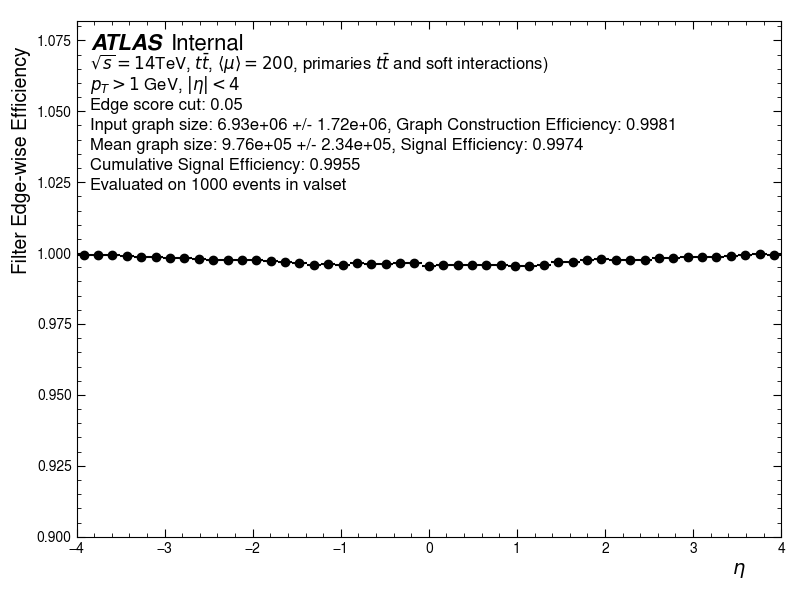
\includegraphics[width=\textwidth]{figures/filter/edgewise_efficiency_with_radius_edgesplits_edgecut_5_eta.png}
    \caption{}
    \label{subfig:filter-eff-eta}
\end{subfigure}
\begin{subfigure}{0.49\textwidth}
    \centering
    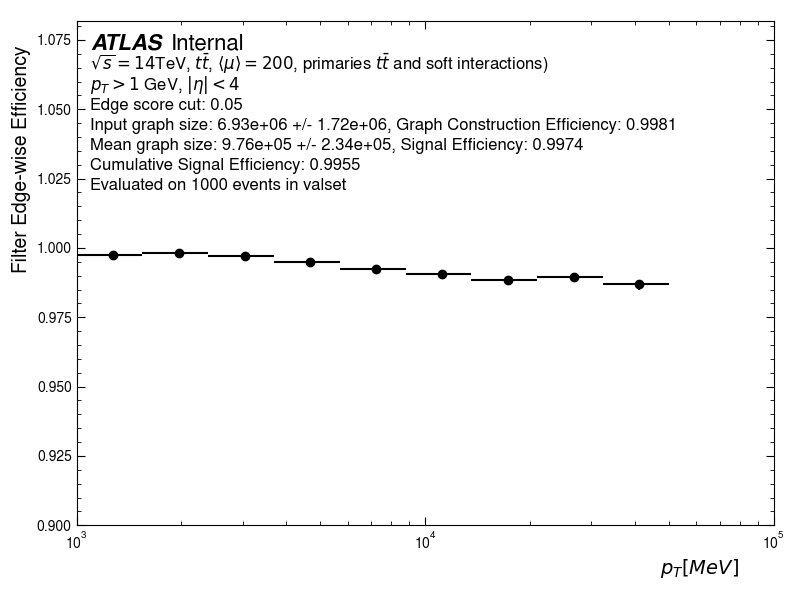
\includegraphics[width=\textwidth]{figures/filter/edgewise_efficiency_with_radius_edgesplits_edgecut_5_pt.png}
    \caption{}
    \label{subfig:filter-eff-pt}
\end{subfigure}
    \caption{Edge efficiency of the Filter network on graphs constructed by the Metric Learning method as a function of $\eta$ (a) and $p_T$ (b).}
    \label{fig:filter-eff-pur-pt-eta}
\end{figure}

Figures \ref{subfig:filter-eff-rz} \ref{subfig:filter-pur-rz} respectively show the edge efficiency and purity as functions of the spherical coordinates $(r,z)$ of the source node. 
These plots illustrate the variation in $\epsilon$ and $\rho$ over the detector volume. 
\ref{subfig:filter-eff-rz} show excellent efficiency throughout the detector. 
Slight efficiency loss is observed in the outermost pixel layer and inner two layers of the strip barrel, where a track transitions between two sensor technologies. 
Overall, the edge efficiency over target particles is $0.996$, i.e. on average 0.4 is lost per 100 target edges.

\begin{figure}[h!]
\begin{subfigure}{\textwidth}
    \centering
    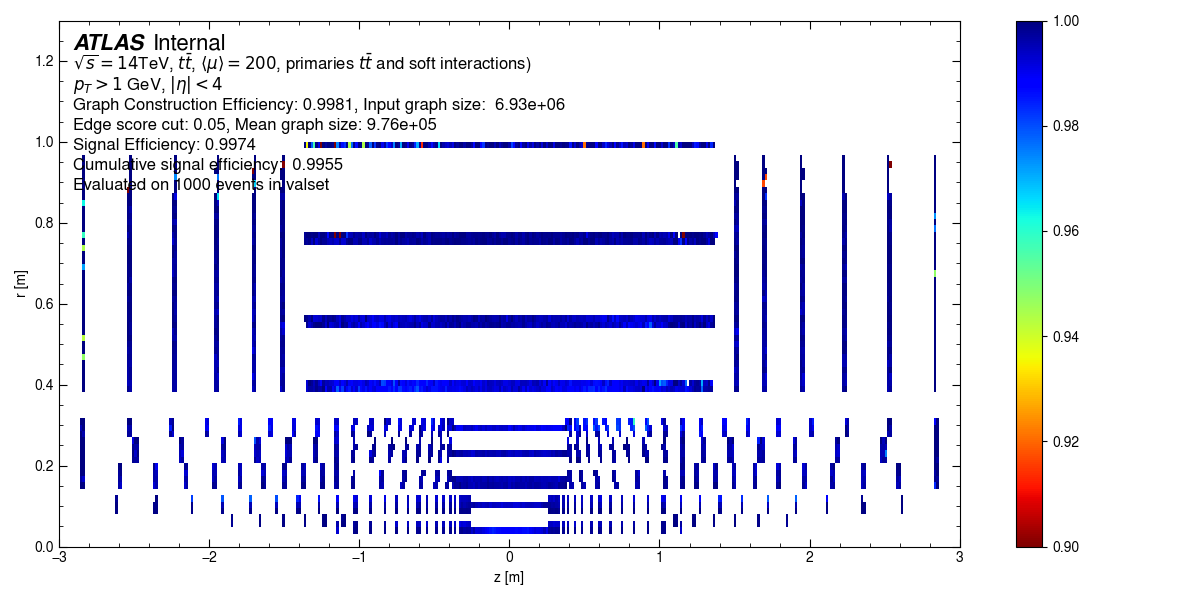
\includegraphics[width=\textwidth, trim={0cm 0 3cm 0}, clip]{figures/filter/cumulative_edgewise_efficiency_rz.png}
    \caption{}
    \label{subfig:filter-eff-rz}
\end{subfigure}
\begin{subfigure}{\textwidth}
    \centering
    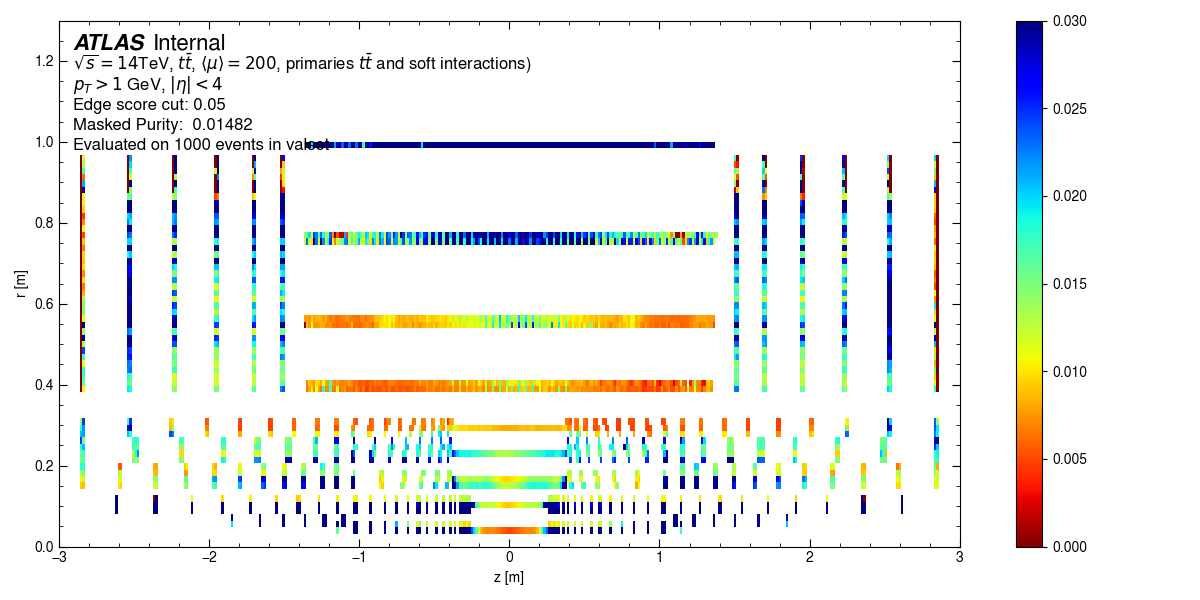
\includegraphics[width=\textwidth, trim={0cm 0 2.85cm 0}, clip]{figures/filter/edgewise_masked_purity_rz.png}
    \caption{}
    \label{subfig:filter-pur-rz}
\end{subfigure}
    \caption{Edge efficiency (a) and purity (b) of the Filter network on graphs constructed by the Metric Learning method as functions of the $(z,r)$-coordinates of the inner hit.}
    \label{fig:filter-eff-pur-rz}
\end{figure}

The average edge purity after filtering is $\rho=1.48\%$, which is not uniform throughout the detector. 
Two regions of low purity are identified. 
The first region with ${\rho}\approx0.4\%$ is located in the innermost pixel layer, closest to the interaction point. 
This proximity leads to a high density of space points, as shown in figure \ref{fig:hit-density-rz}, and consequently a large number of possible random connections. 
% As purity is inversely proportional to the number of connections, this explains observation.
This increases the chance of a misidentified fake edge and leads to low purity.
The second region is located in the transition region between the pixel detector and the strip detector, and between the strip barrel and end-caps. 
Multiple factors play a role in the lowered purity, including (1) changing detector geometry, (2) accumulated material effects, and (3) the presence of single-cluster strip hits. 
A similar performance decrease is observed with the \textbf{Interaction Network} in the same detector region, of which a detailed discussion accounting for both networks will be given in section \ref{subsect:ignn-result}.  

\begin{figure}[h!]
    \centering
    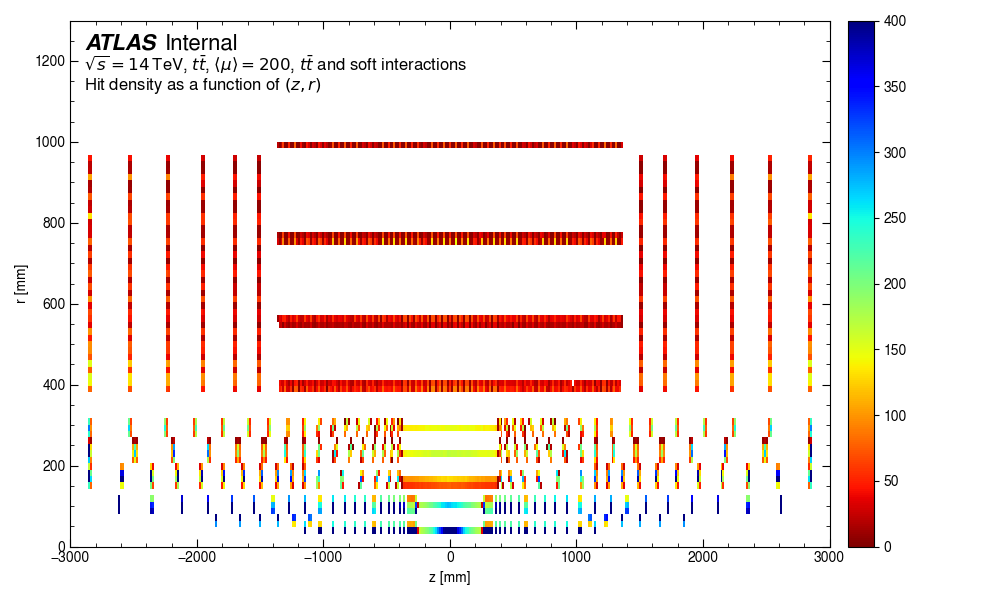
\includegraphics[width=\textwidth, trim={0cm 0 2cm 0}, clip]{figures/hit-density.png}
    \caption{The number of space points per $(z,r)$-bin averaged over 50 $t\bar{t}$ events. The binwidth is 15 mm in both $z$- and $r$-direction.}
    \label{fig:hit-density-rz}
\end{figure}

Although the edge purity remains low, of $\mathcal{O}(1\%)$, the Filter network reduces the average number of edges to $9.76\times 10^5$, $86\%$ smaller than the input graph size of $6.93\times 10^6$, while preserving the high edge efficiency from the graph construction stage.
Recall that the Filter network aims to bring the number of edges down to a reasonable level, so it is more important to avoid falsely rejecting target edges than to eliminate \textit{all} fake edges. 
This mission is reserved for a larger, more sophisticated \ignn introduced in the next section.

\begin{table}[h!]
    \centering
    \begin{tabular}{l|c|c|c}
      Graph Construction Method  & Edge efficiency [\%] & Edge Purity & Number of edges  \\
      \hline \hline
        Module Map \textbf{\textsc{MinMax}} & 99.69 & & $1.22\times 10^6$ \\
        Module Map \textbf{\textsc{MeanRMS}} & 99.51  & & $8.55\times 10^5$ \\
        Metric Learning + Filter & 99.55  & & $9.76\times 10^5$\\
        \hline
    \end{tabular}
    \caption{Comparison of graphs entering the \ignn}
    \label{tab:graph-contruction-comparison}
\end{table}

Table \ref{tab:graph-contruction-comparison} compares properties of graphs produced by Metric Learning and Filter networks to those produced by the Module Map method. 
They all have high edge efficiency, with $\epsilon> 99.5\%$. 
The Module Map with \textsc{MinMax} selection creates edges with $1.2$ million edges, while the other methods yield fewer than 1 million edges. 

\section{The Interaction Network}
\label{sect:ignn}

In the section, a graph neural network is used to identify the majority of fake edges in graphs constructed from either the Module Map technique, or the Metric Learning network.
Graphs from the former are directly subjected to the GNN, whereas those from the latter are passed through a Filter network to reduce ``easy" fake edges beforehand.

\subsection{Methods}

The \ignn~architecture, proposed by Google DeepMind in 2016, 
is used in this thesis \cite{interaction-gnn}. 
It was first successfully applied to the problem of track reconstruction by the \textsc{ExaTrkx} project \cite{exatrkx}, delivering good tracking performance when tested on the Particle Tracking Challenge, or commonly known as the TrackML, dataset \cite{trackml-particle-identification}.
Compared to TrackML, our dataset represents a more realistic and complex detector geometry and thus a greater challenge. 
The \ignn~model architecture has been carefully optimized to deal with this complexity. 

The model can be divided into three components: a set of encoders, a set of convolution modules, and a decoder. In the encoding phase, a node encoder, denoted by $\phi_{enc}: \mathbb{R}^d \rightarrow \mathbb{R}^D$ maps the features $\mathbf{x}_i$ of node $v_i \in V$ to a D-dimensional latent representation $\mathbf{h}_i^0$, such that
\begin{equation}
    \label{eq:10.5}
    \mathbf{h}_i^0 = \phi_{enc}(\mathbf{x}_i).
\end{equation}
Next, an edge encoder $\phi_e:\mathbb{R}^{2\times D + F}\rightarrow \mathbb{R}^D$ maps the latent space node features $(\mathbf{h}_i^0, \mathbf{h}_j^0)$ of nodes $(v_i, v_j)$ connected by an edge $e_{ij}\in E$, and a set of hand-engineered edge features $\mathbf{u}_{ij}\in \mathbb{R}^F$ to an edge feature vector $\mathbf{k}_{ij}^0$,
\beq
\label{eq:10.6}
\mathbf{k}_{ij}^0 = \psi_{enc}([\mathbf{h}_i^0 |\mathbf{h}_j^0|\mathbf{u}_{ij}])
\eeq
The custom edge features, listed in table \ref{tab:gnn-edge-features}, resemble the geometric observables defined for the Module Map edge cuts, making $\mathbf{u}_{ij}$ a 6-dimensional vector.

\begin{table}[h!]
    \centering
    \begin{tabular}{|c|c|}
    \hline
      Feature & Formula \\ \hline\hline
     $\Delta r_{ij}$    & $r_j - r_i$ \\ \hline
     $\Delta \phi_{ij}$ & $\phi_j - \phi_i$ \\ \hline
     $\Delta z_{ij}$ & $z_j - z_i$ \\ \hline
     $\Delta \eta_{ij}$ & $\eta_j - \eta_i$ \\ \hline
     $\phi$-slope & $\frac{\Delta\phi_{ij}}{\Delta r_{ij}}$ \\ \hline
     $r\phi$-slope & $\frac{r_i+r_j}{2}\times \frac{\Delta\phi_{ij}}{\Delta r_{ij}}$ \\ \hline \hline
    \end{tabular}
    \caption{Hand-engineered edge features}
    \label{tab:gnn-edge-features}
\end{table}

The most important component of the \ignn~is the graph convolution modules $\{\varphi^l\}_{l=1}^L$. 
They evolve the encoded node and edge features over $L$ iterations by taking into account the graph connectivity. 
At each iteration $l$, the node feature $\mathbf{h}_i^l$ of node $v_i$ is computed from its feature from the previous step $\mathbf{h}_i^{l-1}$, and a message vector $\mathbf{m}_i^{l}$ containing information from other nodes directly connected to $v_i$. 
First, the latent feature vectors $k_{ij}^{l-1}$ of edges connecting to $v_i$ are aggregated to generate a vector $\mathbf{m}_{i \leftarrow}^l$
\beq
\label{eq:10.7}
\mathbf{m}_{i \leftarrow}^l = \textsc{Aggregate}(\{\mathbf{k}_{ji}^{l-1}\, \forall e_{ji} \in E\}),
\eeq
and then the aggregation is repeated on edges connecting from $v_i$ to create a vector $\mathbf{m}_{i \rightarrow}^l$
\beq
\label{eq:10.8}
\mathbf{m}_{i \rightarrow}^l = \textsc{Aggregate}(\{\mathbf{k}_{ij}^{l-1}\, \forall e_{ij} \in E\}).
\eeq
The message vector $\mathbf{m}_i^{l}$, simply
\beq
\label{eq:10.9}
\mathbf{m}_{i}^l = \left[\mathbf{m}_{i \leftarrow}^l | \mathbf{m}_{i \rightarrow}^l  \right],
\eeq
is used to update the node vector by 
\beq
\label{eq:10.10}
\mathbf{h}_i^l = \varphi_v^l(\mathbf{h}_i^{l-1}, \mathbf{m}_{i}^l),
\eeq
and the updated node vector is then used to update the edge vector
\beq
\label{eq:10.11}
\mathbf{k}_{ij}^l = \varphi_e^l(\mathbf{k}_{ij}^{l-1}, \mathbf{h}_i^l, \mathbf{h}_j^l).
\eeq

Equations \eqref{eq:10.7}-\eqref{eq:10.11} describe the message passing mechanism of the \ignn, which, analogous to the \graphsage~mechanism of the Filter network, leverages the connectivity on which the graph is defined to evolve the node vectors. 
% While we could feed the graph to a fully-connected network (FCN), and this is indeed what we do with the node encoder $\phi_{enc}$, it treats each node as an individual entry in a table and makes predictions based solely on its features, ignoring those of other nodes. 
% On the other hand, thanks to the message passing mechanism, over the same set of nodes, the graph topology enters the node and edge evolution via the \textsc{Aggregate} functions. 
% Different graph topologies, defined by different sets of edges, thus yield different node representation in the end, enhancing the network's expressive power. 

\begin{algorithm}
\caption{Message passing mechanism of the \ignn }\label{alg:ignn-message-passing}
\For{$l \in \{1,\dotsc , L\}$}{
  $\mathbf{m}_{i \leftarrow}^l \gets \textsc{Aggregate}(\{\mathbf{k}_{ji}^{l-1}\, \forall e_{ji} \in E\})$; \\
  $\mathbf{m}_{i \rightarrow}^l \gets \textsc{Aggregate}(\{\mathbf{k}_{ij}^{l-1}\, \forall e_{ij} \in E\})$; \\
  $\mathbf{m}_{i}^l \gets \left[\mathbf{m}_{i \leftarrow}^l | \mathbf{m}_{i \rightarrow}^l  \right]$; \\
  $\mathbf{h}_i^l \gets \varphi_v^l(\mathbf{h}_i^{l-1}, \mathbf{m}_{i}^l)$; \\
  $\mathbf{k}_{ij}^l \gets \varphi_e^l(\mathbf{k}_{ij}^{l-1}, \mathbf{h}_i^l, \mathbf{h}_j^l)$;
}
\end{algorithm}

However, different from \graphsage, the message passing mechanism of the \ignn~tracks the edge vector and treats it as the message between nodes.
Indeed, very few other GNN architectures maintain edge-level intermediate vectors, since information exchange between nodes can be effectuated without and explicit edge state. 
Because the number of edges in a graph is generally much larger than the number of nodes, tracking the gradient of an edge-level network, such as the edge updater $\varphi_v^j$, consumes more memory than that of node-level networks.
However, the increased computational cost is justified by better expressivity. 
Reference \cite{interaction-gnn} proposed the \ignn~to model a multi-body physical system, in which each node represents an object and each edge the interaction between these objects. 
As such, the node vector represents the physical state of each object, and the edge vector quantifies the effect an object has on another's hidden state. 
So naturally, the object state vector evolves with its previous state and the interaction as input, as seen on equation \eqref{eq:10.10}.
This interaction itself depends not only on the current object state, but also on its history, so the edge updater uses its previous state, and the current object state, as seen in equation \eqref{eq:10.11}.

The accuracy of the \ignn~in modelling multi-body physical systems observed by reference \cite{interaction-gnn} lends evidence to the effectiveness of explicitly tracking edge-level features following this physics intuition.
In it unclear, however, how far this logic could be extended to other problems, or in reverse, how closely the track pattern recognition problem resembles an $n$-body system. 
For example, it is conceivable that since a track traces the evolution of a particle through the detector, hits from inner layers (the past) provide useful information to predict whether a hit in an outer layer (the future) belongs to the track, and vice versa. 
In this sense, the interaction between two hits, when evolved over multiple steps, encodes the properties of a track formed from themselves and other hits among which they exchange information. 
The network can then learn to distinguish true and fake edges by picking the most probable path given the hits on a particular search road.
This intuition is in no way a \textit{proof}. 
Deep neural networks are after all blackbox algorithms, whose explainability awaits further developments and lies outside the scope of this thesis.
We contend with the assumption that the \ignn's success on a simplified tracking problem (TrackML) \cite{exatrkx} holds potentials for a more realistic counterpart (ATLAS ITk), if given sufficient training data and optimization. 

In the final stage, the edge vector $\mathbf{k}_{ij}^L$ is fed to a decoder $\psi_{dec}:\mathbb{R}^D\rightarrow [0,1]$ to compute a single number interpreted as the probability of being a true edge. 
\beq
\label{eq:10.12}
\hat{y}_{ij} = \psi_{dec}(\mathbf{k}_{ij}^L)
\eeq
The \ignn~architecture is summarized in algorithm \ref{alg:ignn}. The hidden dimension of all latent-space vectors is set to $D=128$. A simple element-wise average is used as the aggregation function 
\begin{equation}
    \label{eq:10.13}
    \textsc{Aggregate}\left( \{ \mathbf{k}_{ij} \}_{j=1} ^ {N} \right) = \frac{1}{N} \sum_{i=1} ^N \mathbf{k}_{ij}.
\end{equation}
The message passing mechanism is carried out over $L=8$ iterations, each with a distinct set of node and edge updaters. All neural network submodules in the model are MLPs consisting of 3 layers, each containing $M=128$ neurons. 

\begin{algorithm}
\caption{The \ignn }\label{alg:ignn}
Given input graph $G(V,E)$, input node feature $\mathbf{x}_i\, \forall v_i \in V$, \\
$\mathbf{h}_i^0\gets \phi_{enc}(\mathbf{x}_i)$;\\
$\mathbf{k}_{ij}^0 \gets \psi_{enc}(\mathbf{h}_i^0, \mathbf{h}_j^0)$;\\
\For{$l \in \{1,\dotsc , L\}$}{
  $(\mathbf{h}_i^l, \mathbf{k}_{ij}^l) \gets \varphi(\mathbf{h}_i^{l-1}, \mathbf{k}_{ij}^{l-1}, \{\mathbf{k}_{ij}^{l-1}\, \forall e_{ij} \in E \}, \{\mathbf{k}_{ji}^{l-1}\, \forall e_{ji} \in E\}) $
}
$\hat{y}_{ij} = \psi_{dec}(\mathbf{k}_{ij}^L)$
\end{algorithm}

The model weights are optimized on the edge classification objective, using the weighted binary cross-entropy loss described in equation \eqref{eq:10.2}. Other hyperparameters related to model training are detailed in table \ref{tab:ignn-specification}.

\begin{table}[h!]
    \centering
    \begin{tabular}{l|l}
    \hline
      Hyperparameter   &  Value \\ \hline 
      Number of message passing operations & 8 \\
        Hidden dimension & 128 \\
      Hidden activation functions & \relu \\
       Optimizer & \textsc{Adam} \\
       Learning rate & 0.001 \\
       Epochs & $\approx 200$ \\
    \hline
    \end{tabular}
    \caption{\ignn~model specification}
    \label{tab:ignn-specification}
\end{table}

\subsection{Results}
\label{subsect:ignn-result}

% \begin{figure}[htbp]
% \centering
% \begin{subfigure}[b]{0.49\textwidth}
%     \centering
%     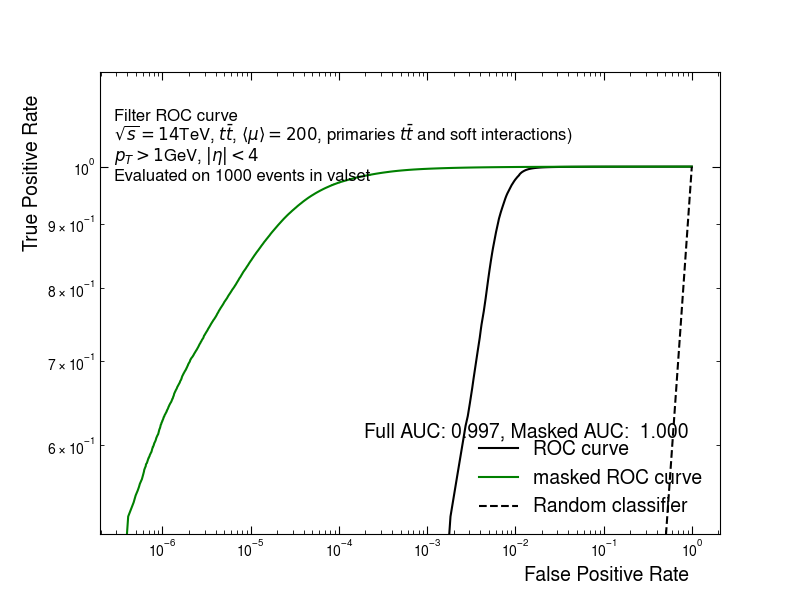
\includegraphics[width=\textwidth]{figures/gnn-meanrms/gnn_MM_UNCLEANED_MEANRMS_WITHOUT_CONCAT_LATENT128_LN/roc_curve.png}
%     \caption{}
%     \label{subfig:gnn-roc-meanrms}
% \end{subfigure}
% \begin{subfigure}[b]{0.49\textwidth}
%     \centering
%     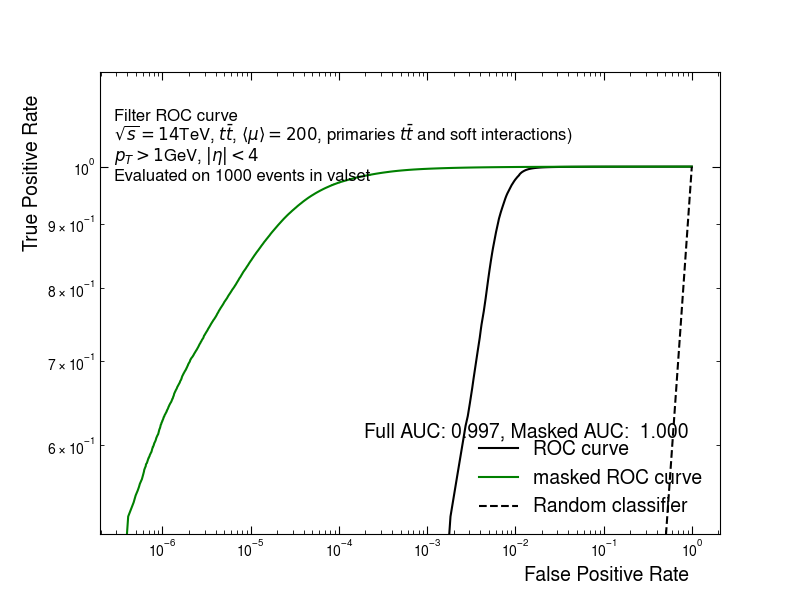
\includegraphics[width=\textwidth]{figures/gnn-meanrms/gnn_MM_UNCLEANED_MEANRMS_WITHOUT_CONCAT_LATENT128_LN/roc_curve.png}
%     \caption{}
%     \label{subfig:gnn-roc-ml}
% \end{subfigure}
% \caption{Caption}
% \label{fig:gnn-roc-meanrms-ml}
% \end{figure}

Being both edge-classifying graph neural networks, the Filter and the Interaction network are evaluated using the same metrics. 
Figure \ref{fig:gnn-eff-eta-pt-meanrms-ml}shows the edge efficiency of the \ignn~ as a functions of the particle's pseudorapidity (left) and transverse momentum (right). 
Figures \ref{subfig:gnn-eff-eta-meanrms} and \ref{subfig:gnn-eff-pt-meanrms} describes the performance on graphs from the Module Map MeanRMS variant, whereas figures \ref{subfig:gnn-eff-eta-ml} and \ref{subfig:gnn-eff-pt-ml} those from the Metric Learning variant.
The Module Map MinMax and MeanRMS variants have similar performance, so the former is omitted from all following figures in this chapter for brevity.
The standard edge score cut $0.5$ is applied to make the binary prediction.
Note, however, that this simple score cut will not be used to construct the final track candidate, as described in chapter \ref{chap:track-building}.

\begin{figure}[h!]
\centering
\begin{subfigure}[b]{0.49\textwidth}
    \centering
    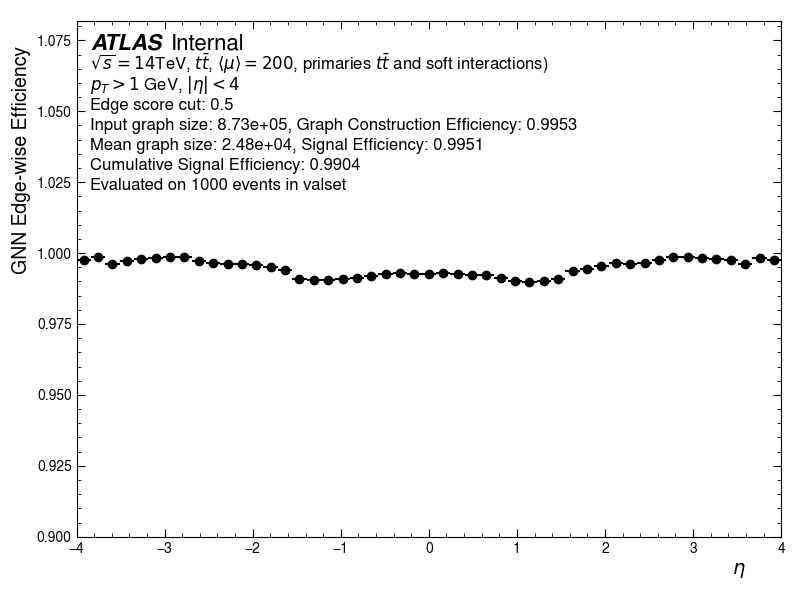
\includegraphics[width=\textwidth]{figures/gnn_MM_UNCLEANED_MEANRMS_WITHOUT_CONCAT_LATENT128_LN/edgewise_efficiency_eta.png}
    \caption{}
    \label{subfig:gnn-eff-eta-meanrms}
\end{subfigure}
\begin{subfigure}[b]{0.49\textwidth}
    \centering
    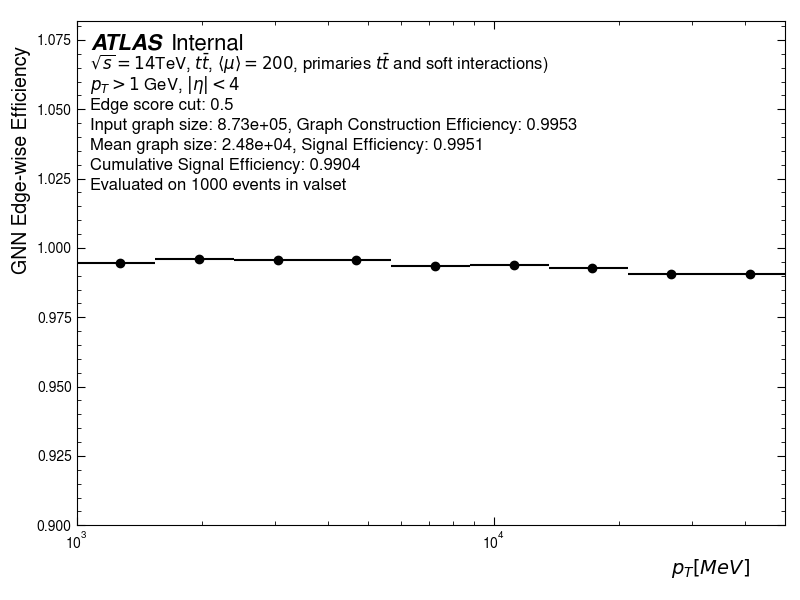
\includegraphics[width=\textwidth]{figures/gnn_MM_UNCLEANED_MEANRMS_WITHOUT_CONCAT_LATENT128_LN/edgewise_efficiency_pt.png}
    \caption{}
    \label{subfig:gnn-eff-pt-meanrms}
\end{subfigure}

\begin{subfigure}[b]{0.49\textwidth}
    \centering
    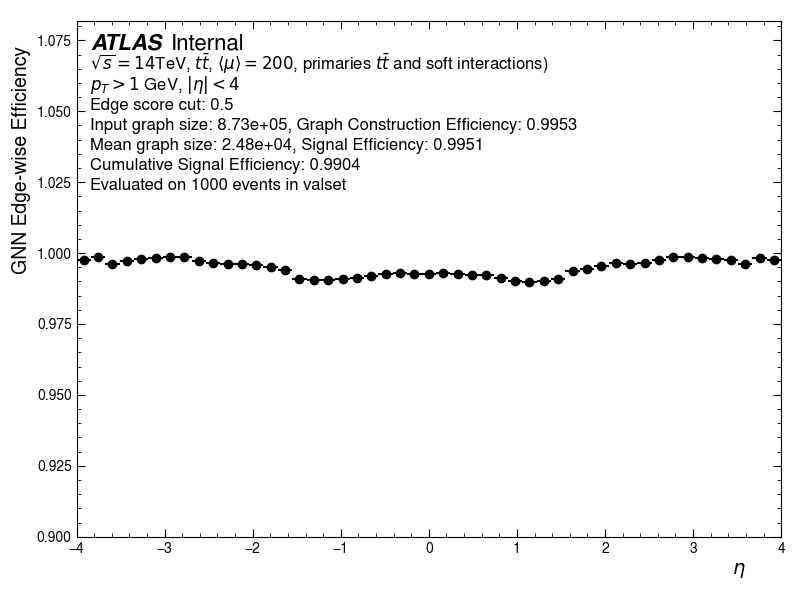
\includegraphics[width=\textwidth]{figures/gnn_MM_UNCLEANED_MEANRMS_WITHOUT_CONCAT_LATENT128_LN/edgewise_efficiency_eta.png}
    \caption{}
    \label{subfig:gnn-eff-eta-ml}
\end{subfigure}
\begin{subfigure}[b]{0.49\textwidth}
    \centering
    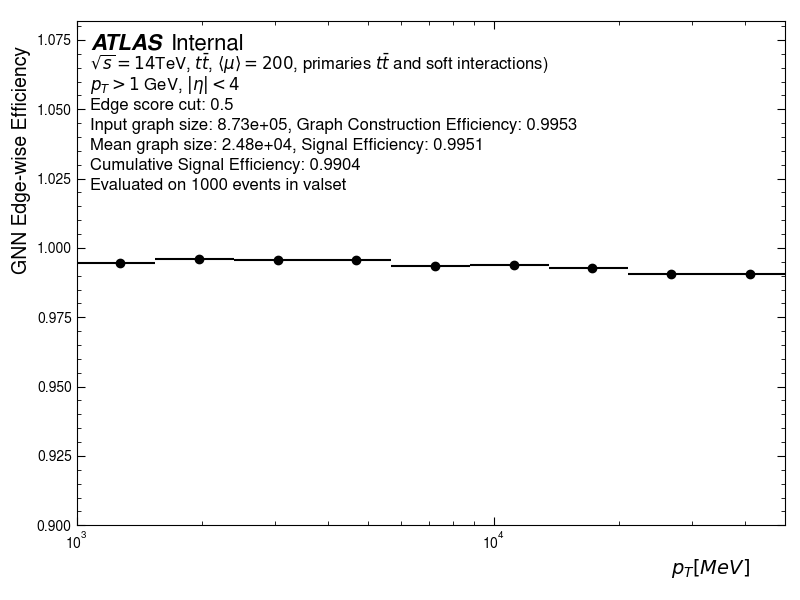
\includegraphics[width=\textwidth]{figures/gnn_MM_UNCLEANED_MEANRMS_WITHOUT_CONCAT_LATENT128_LN/edgewise_efficiency_pt.png}
    \caption{}
    \label{subfig:gnn-eff-pt-ml}
\end{subfigure}
\caption{Edge efficiency of the \ignn~as a function of $\eta$ (left) and $p_T$ (right), evaluated on graphs created using the Module Map method with MeanRMS (upper) and MinMax selections (lower). }
\label{fig:gnn-eff-eta-pt-meanrms-ml}
\end{figure}

The \ignn~achieves efficiency exceeding 99.5\% on graphs constructed by both the Module Map and Metric Learning techniques.
The performance is also consistently higher than 99\% throughout the detector.
% The edge efficiency of the \ignn~on graphs constructed by the Module Map MeanRMS method exceeds 99\% throughout the detector.
Against the truth transverse momentum, a slight dip in efficiency is observed at high $p_T$.
As we have seen from the discussion on the Filter network, the combination of low training statistics and different curvature means that edges from high-$p_T$ tracks receive less attention during training. 
As a result, the model favours the more abundant low-$p_T$ track edges and more often misidentifies high-$p_T$ ones.
Since high-$p_T$ tracks are more concentrated in the barrel region, a slight decrease in efficiency is observed in $\abs{\eta}<1.5$.

It is worth noting that the GNN4ITk pipeline has been developed over several iterations of MC data, the most recent of which is described in reference \cite{ctd23-gnn4itk}, on a dataset of 1780 $t\bar{t}$-events.
The cumulative edge efficiency achieved in this thesis is 99.04\% for the \textbf{MeanRMS} variant, higher than the previous result of 98.2\%.
The enhanced performance can be attributed to an optimized model architecture, and a larger training dataset, in particular 7800 event versus 1600 in reference \cite{ctd23-gnn4itk}. 

\begin{figure}[h!]
    \centering
    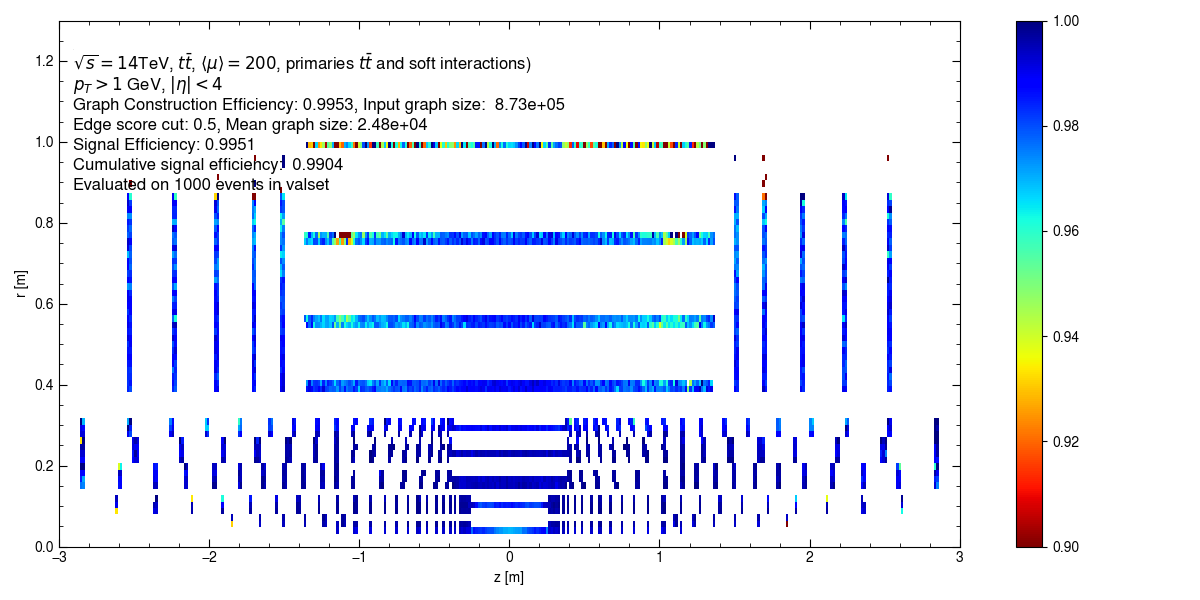
\includegraphics[width=\textwidth, trim={0cm 0 2.85cm 0}, clip]{figures/gnn-meanrms/gnn_MM_UNCLEANED_MEANRMS_WITHOUT_CONCAT_LATENT128_LN/cumulative_gnn_edgewise_eff_rz_check.png}
    \caption{Edge efficiency of the \ignn~on graphs constructed by the \textbf{Module Map MeanRMS} as a function of the $(z,r)$-coordinates of the inner hit.}
    \label{fig:gnn-eff-rz}
\end{figure}

The edge efficiency as a function of the $(z,r)$-coordinates of the inner hit, shown in figure \ref{fig:gnn-eff-rz}, illustrates the spatial distribution of misidentified true edges. 
Similar to the case of the Filter network, pockets of edge inefficiency as low as 96\% are observed on the outermost pixel layer and near the edges of barrel strip layers, where a trajectory passes from one sensor technology or geometry to another. 
It is clear that both graph neural networks perform better in the pixel detector than in the the strip detector. 
The degraded performance can be attributed to a number of factors. 
First, accumulated material effects change the geometry of the orbit and increase the chance of an edge deviating from the pattern observed on the inner layers and being deemed incompatible with other true edges.
Second, the transition between one sensor technology to another creates heterogeneity in both the geometric representation of the local coordinates, which is part of the input features and their resolution, as described in section \ref{sect:cluster-spacepoint}.
Yet despite the inherently heterogeneous data, all models employed in this thesis are homogeneous in architecture, which, though generally sufficient for their purpose, cannot predict well the cases where the heterogeneity can provide useful discrimination. 
Third, the hit inefficiency in space point formation, also described in section \ref{sect:cluster-spacepoint}, means that true particle tracks are more likely to pass a strip layer without a hit when constructed from space points.
Learning from these tracks, the GNNs may tolerate or even encourage layer-skipping edges in the strip detector, at the detriment of some true edges not well featured in the training data.
We will return to the third issue in chapter \ref{chap:tracking-performance}, as it has an even larger implication on the tracking performance. 
In general, the training input data into the GNN4ITk contains shortcomings that are not optimal for learning and processing the output track candidates, to be addressed in future work.

\begin{figure}[h!]
    \centering
    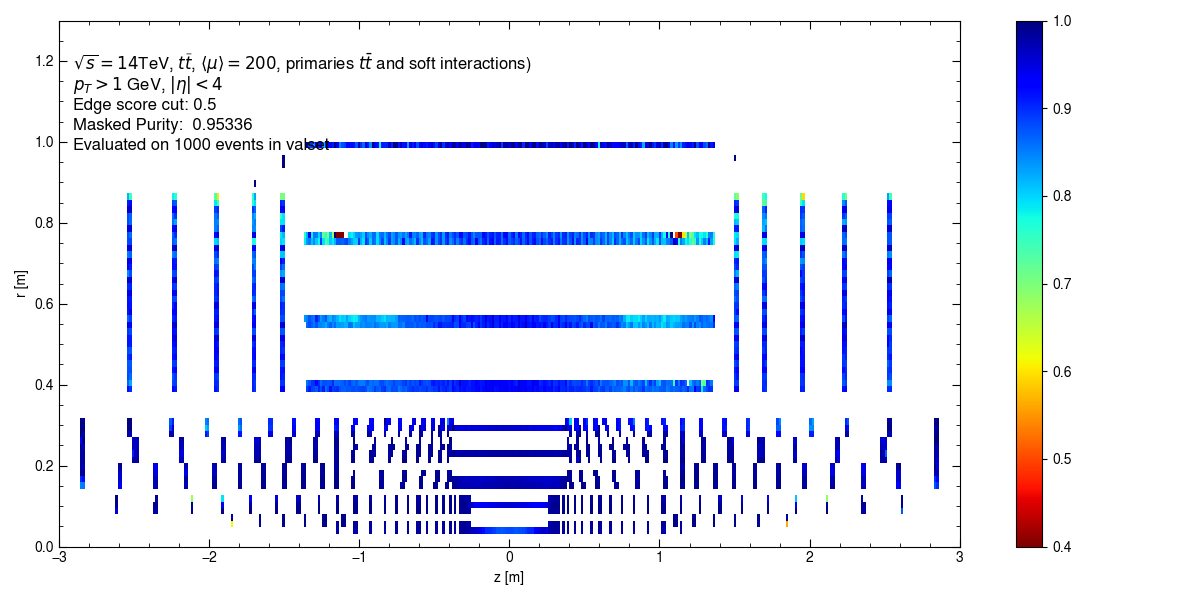
\includegraphics[width=\textwidth, trim={0cm 0 2.85cm 0}, clip]{figures/gnn-meanrms/gnn_MM_UNCLEANED_MEANRMS_WITHOUT_CONCAT_LATENT128_LN/gnn_edge_wise_pur_rz_check_masked_purity_rz.png}
    \caption{Edge purity of the \ignn~on graphs constructed by the \textbf{Module Map MeanRMS} as a function of the $(z,r)$-coordinates of the inner hit.}
    \label{fig:gnn-pur-rz}
\end{figure}

The edge purity as a function of the $(z,r)$-coordinates of the inner hit, shown in figure \ref{fig:gnn-pur-rz}, paints a similar picture as the efficiency distribution.
On graphs from the MeanRMS variant, an average purity of 95.3\% is achieved with noticeable variations over the detector regions.
% The MeanRMS variant of the GNN4ITk achieves an overall purity of 95.3\% is achieved by the \textbf{MeanRMS} variant, whose spatial distribution is unevent.
Model predictions are more pure in the pixel detector than in the strip detector, with pockets of impurity as high as 25\% at the edges of the strip barrel. 
When compared to the input graphs, which average to $\rho <0.1\%$ and $\mathcal{O}(10^6)$ edges in all variants (see table \ref{tab:graph-contruction-comparison}), a purity level of $\sim 95\%$ in graphs of $\mathcal{O}(10^4)$ edges represents a significant rate of fake rejection. 
Nevertheless, the residual impurity creates challenges to the construction of track candidates, which is the focus of chapter \ref{chap:track-building}.

\begin{table}[h!]
    \centering
    \begin{tabular}{l|c|c|c}
      Graph Construction Method  & Edge efficiency [\%] & Edge Purity & Number of edges  \\
      \hline \hline
        Module Map \textbf{\textsc{MinMax}} & 99.40 & 95.64 & $2.53\times 10^4$ \\
        Module Map \textbf{\textsc{MeanRMS}} & 99.04  & 95.34 & $2.48\times 10^4$ \\
        Metric Learning + Filter & 99.55  & & $9.76\times 10^5$\\
        \hline
    \end{tabular}
    \caption{Performance of the \ignn~across three graph construction methods. }
    \label{tab:edge-classification-comparison}
\end{table}

A comparison in performance of the three GNN4ITk variants is provided in table \ref{tab:edge-classification-comparison}.
The {Module Map MinMax} variant displays the best performance in both efficiency and purity, followed by the MeanRMS and the Metric Learning variants.
% Although these edge-based metrics are useful in evaluating and optimizing machine learning models, 
The edge-based efficiency and purity are useful in developing machine learning models. 
However, in production settings, the performance must be evaluated using Athena \cite{atlas_collaboration_2021_4772550}, the main software analysis framework of ATLAS.
% However, these edge-based metrics are useful to evaluate and optimize model design, but to assess the algorithm in production settings, the tracking and computing performance are more relevant in the larger context of ATLAS event reconstruction.

As such, the next step of the GNN4ITk pipeline partitions a graphs whose edges have been scored by the GNN into track candidates, which are then fed into Athena. 
Track parameters are estimated and other important metrics are computed in a unified framework for both the CKF- and the GNN-based track finders.
The graph segmentation step is presented in the next chapter, and the tracking performance in chapter \ref{chap:tracking-performance}.

% Overall, good efficiency 
